%%
% La siguiente plantilla esta basada en el siguiente enlace:
% http://academic.reed.edu/physics/courses/Physics332.s08/reports.html
% La plantilla original puede descargarse de ese sitio
% Se dejo parte del texto original en inglés para ilustar el uso de la plantilla
% Se hicieron algunas modificaciones para ajustar el idioma y otros detalles para 
% completar un reporte técnico breve pero muy puntual
% Modificación Inicial: Marco Aurelio Nuno Maganda - 11/SEP/2014
% 
% Enlace a la documentación del tipo de documento base (revtex4)
% http://mirror.hmc.edu/ctan/macros/latex/contrib/revtex/doc/latex/revtex/source/revtex4-1.pdf
%
% En algunas distribuciones es necesario instalar el paquete texlive-publishers
%
%\documentclass[letterpaper,aps,twocolumn,pre,nofootinbib]{revtex4}
%\documentclass[twocolumn]{article}
\documentclass[conference]{IEEEtran}

\usepackage[spanish]{babel}
\usepackage{amsmath,amssymb,amsfonts,amsthm}
\usepackage{graphicx}
%\usepackage{bbm}
\usepackage[utf8]{inputenc} % Caracteres en Español (Acentos, ñs)
\usepackage{url} % ACENTOS
\usepackage{hyperref} % Referencias
\usepackage{subfig}
\usepackage{lipsum}
\usepackage{balance}


\usepackage{graphicx} % Required for including images
\usepackage[font=small,labelfont=bf]{caption} % Required for specifying captions to tables and figures


\usepackage{tikz}
\usetikzlibrary{automata, positioning, arrows}

%%%%%%%%%%%%%%%%%%%%%%%%%%%%%%%%%%%%%%%%%%%%%
% PARCHE PARA ELIMINAR LA FECHA DEL DOCUMENTO
% 
\usepackage{etoolbox}
\makeatletter
% \frontmatter@RRAP@format is responsible for the parentheses
\patchcmd{\frontmatter@RRAP@format}{(}{}{}{}
\patchcmd{\frontmatter@RRAP@format}{)}{}{}{}
%\renewcommand\Dated@name{}
\makeatother	
% FIN DEL PARCHE
% 
%%%%%%%%%%%%%%%%%%%%%%%%%%%%%%%%%%%%%%%%%%%%%

%%%%%%%%%%%%%%%%%%%%%%%%%%%%%%%%%%%%%%%%%%%%%
% PARCHE PARA PERMIRIR UTILIZAR BIBLATEX EN ESTA PANTLLA
%\PassOptionsToPackage{square,numbers}{natbib}
%\RequirePackage{natbib}  
%%%%%%%%%%%%%%%%%%%%%%%%%%%%%%%%%%%%%%%%%%%%%

\usepackage[backend=bibtex,sorting=none]{biblatex}
% Estas lineas permiten romper los hipervinculos muy largos !!!!
\setcounter{biburllcpenalty}{7000}
\setcounter{biburlucpenalty}{8000}
\addbibresource{references.bib}

% Actualiza en automático la fecha de las citas de internet a la fecha de la compilación del documento
\usepackage{datetime}
\newdateformat{specialdate}{\twodigit{\THEDAY}-\twodigit{\THEMONTH}-\THEYEAR}
\date{\specialdate\today}

% la sentencia \burl en las citas... 
\usepackage[hyphenbreaks]{breakurl}

\renewcommand\spanishtablename{Tabla}
\renewcommand\spanishfigurename{Figura}



\begin{document}

\newcommand{\breite}{0.9} %  for twocolumn
\newcommand{\RelacionFiguradoscolumnas}{0.9}
\newcommand{\RelacionFiguradoscolumnasPuntoCinco}{0.45}



\title{Reporte Individual 3 \\Background Removal}

\author{\IEEEauthorblockN{Manzano Estrada Vanessa Nataly\IEEEauthorrefmark{1},
Medina Cavazos Luis Alejandro\IEEEauthorrefmark{1} y 
Moreno Ledesma Ximena Abigail\IEEEauthorrefmark{1}}
\IEEEauthorblockA{Ingeniería en Tecnologías de la Información\\
Universidad Politécnica de Victoria}
}
\maketitle



\begin{abstract} 

    En este documento se presenta el desarrollo de una aplicación Android que realiza segmentación en tiempo real de personas en imágenes y video, utilizando CameraX para la captura de la cámara, ML Kit Selfie Segmentation para generar máscaras de segmentación, y Jetpack Compose para la interfaz de usuario. La aplicación permite seleccionar una imagen desde la galería y, posteriormente, combinarla con la persona detectada en la cámara frontal. Se realizaron pruebas para validar que la segmentación y el reemplazo de fondo funcionen correctamente, mostrando la persona en primer plano sobre el fondo seleccionado.

\end{abstract}



\section{Introducción}

    La segmentación de imágenes es una técnica fundamental en el campo de la visión por computadora, permitiendo la identificación y separación de objetos dentro de una imagen. En aplicaciones móviles, esta tecnología se utiliza para mejorar la experiencia del usuario mediante efectos visuales avanzados, como el reemplazo de fondos en tiempo real.En este contexto, Google ha desarrollado ML Kit, un conjunto de herramientas de aprendizaje automático que facilita la implementación de funcionalidades como la segmentación de selfies en dispositivos Android. Esta API permite separar al usuario del fondo en tiempo real, utilizando modelos optimizados para dispositivos móviles \cite{mlkit_selfie_segmentation}.

    Por otro lado, Jetpack Compose es un moderno kit de herramientas de UI para Android que simplifica la creación de interfaces de usuario declarativas y reactivas. Su integración con CameraX, una biblioteca que facilita el uso de la cámara en aplicaciones Android, permite el desarrollo de aplicaciones con capacidades avanzadas de captura y procesamiento de imágenes \cite{cameraX_docs}.

    Este proyecto tiene como objetivo el desarrollo de una aplicación Android que combine ML Kit, CameraX y Jetpack Compose para realizar segmentación en tiempo real de personas en imágenes y video. La aplicación permite seleccionar una imagen de fondo desde la galería y, posteriormente, mostrarla detrás de la persona detectada en la cámara frontal. Se implementa un flujo de procesamiento que convierte los frames de la cámara de formato YUV a Bitmap RGB, aplica la segmentación y renderiza el resultado en tiempo real \cite{mlkit_selfie_segmentation}. Además, se utiliza Jetpack Compose para la construcción de la interfaz de usuario, aprovechando sus ventajas en términos de declaratividad y reactividad \cite{compose_docs}.

    La herramienta desarrollada ofrece una experiencia interactiva, permitiendo al usuario visualizar en tiempo real cómo su imagen se combina con diferentes fondos seleccionados. Se realizaron pruebas para validar que la segmentación y el reemplazo de fondo funcionen correctamente, mostrando la persona en primer plano sobre el fondo seleccionado sin errores.

 
\section{Desarrollo Experimental} 
Para la implementación del proyecto, se desarrolló una aplicación móvil en \textbf{Kotlin}, utilizando \textbf{Jetpack Compose} para la interfaz gráfica, junto con \textbf{CameraX} y \textbf{ML Kit de Google} para aplicar segmentación en tiempo real con efectos de fondo virtual.  

Inicialmente se exploró el uso de \textbf{Fritz AI}, siguiendo el tutorial ``Image Segmentation for Android — Smart Background Replacement with Fritz AI'' \cite{fritz}. Dicho recurso proponía el uso del Fritz SDK para generar máscaras segmentadas y reemplazar fondos en imágenes, sin embargo, se determinó que las librerías utilizadas estaban obsoletas y sin soporte, lo que imposibilitaba su uso en entornos actuales de Android.  

Ante esta limitación, se consultó un tutorial en Python sobre segmentación en tiempo real \cite{ytseg}, el cual sirvió de inspiración para la lógica general. Debido a que estaba enfocado en otro lenguaje, se realizó la adaptación completa hacia \textbf{Kotlin} y \textbf{Jetpack Compose}, logrando implementar el procesamiento en dispositivos móviles Android.  

\subsection{Fase 1 – Selección de Imagen de Fondo}
Se implementó la selección de imagen mediante \texttt{ActivityResultContracts.GetContent()}, permitiendo al usuario elegir un archivo de tipo \texttt{image/*}. La imagen fue convertida a un objeto \texttt{Bitmap} en formato \textbf{ARGB\_8888}, asegurando compatibilidad con los procesos posteriores.  

Este procedimiento se apoyó en prácticas descritas en literatura especializada sobre programación móvil \cite{bignerdandroid}.  

\subsection{Fase 2 – Gestión de Permisos}
Antes de iniciar la cámara, fue necesario implementar la gestión de permisos en tiempo de ejecución. Para ello se utilizó \texttt{checkSelfPermission()} y, en caso de ser necesario, se solicitó el permiso de cámara mediante \texttt{ActivityResultContracts.RequestPermission()}.  

El correcto manejo de permisos se documenta ampliamente en textos de desarrollo Android \cite{bignerdandroid}, reforzando la importancia de la seguridad y la interacción usuario-sistema en aplicaciones móviles.  

\subsection{Fase 3 – Captura de Imágenes con CameraX}
Para la captura de imágenes se integró \textbf{CameraX}, utilizando \texttt{ImageAnalysis} con la estrategia \texttt{STRATEGY\_KEEP\_ONLY\_LATEST} a fin de procesar únicamente el frame más reciente y optimizar rendimiento. El análisis de cámara se ejecutó en un \texttt{Executor} independiente, evitando bloqueos en la interfaz.  

La arquitectura recomendada para este tipo de integración se encuentra descrita en guías de desarrollo con Kotlin \cite{bignerdkotlin}.  

\subsection{Fase 4 – Conversión YUV a RGB}
Las imágenes capturadas por la cámara se reciben en formato \textbf{YUV}, el cual no es adecuado para procesamiento directo en \textbf{ML Kit}. Para resolverlo, se implementó una clase utilitaria \texttt{YuvToRgbConverter}, que transforma YUV a \texttt{Bitmap} RGB mediante \texttt{YuvImage} y \texttt{compressToJpeg}.  

Este proceso de conversión se apoyó en fundamentos descritos en bibliografía de visión por computadora aplicada a Android \cite{mlkitbook}.  

\subsection{Fase 5 – Segmentación y Composición de Imágenes}
La segmentación en tiempo real se realizó con \textbf{ML Kit Selfie Segmentation} en modo \texttt{STREAM\_MODE}. El modelo generó una máscara probabilística, la cual fue utilizada para combinar dinámicamente el primer plano (usuario) y el fondo elegido:  

\begin{itemize}
    \item Si el valor de la máscara era mayor a 0.5, se mantenía el píxel de la cámara.  
    \item En caso contrario, se utilizaba el píxel del fondo.  
\end{itemize}

Este tipo de integración práctica entre ML Kit y Kotlin ha sido explorada en distintos textos \cite{mlkotlin}.  

\subsection{Fase 6 – Visualización con Jetpack Compose}
El resultado de la segmentación se desplegó en la interfaz de usuario mediante el componente \texttt{Image} de Jetpack Compose. Se utilizaron mecanismos de estado (\texttt{remember}, \texttt{mutableStateOf}) para refrescar dinámicamente la vista con cada nuevo frame procesado.  

El uso de \textbf{Jetpack Compose} como motor de interfaz declarativa se fundamentó en guías modernas de desarrollo UI en Android \cite{bignerdkotlin, jetpackbook}.  


\section{Resultados} 
Tras integrar cada uno de los módulos principales del sistema, incluyendo la captura de imágenes mediante la cámara del dispositivo, la selección de fondos personalizados desde la galería y la aplicación de segmentación de personas, se obtuvo una aplicación funcional que cumple con los objetivos planteados.

En la \textcolor{red}{\autoref{fig:s1}} se observa la primera interacción con la aplicación, donde el sistema solicita al usuario los permisos necesarios para el uso de la cámara y el acceso a los archivos multimedia del dispositivo. Este paso asegura el correcto funcionamiento de las funciones de captura y almacenamiento.\newpage


\begin{figure}[htbp]
\centering
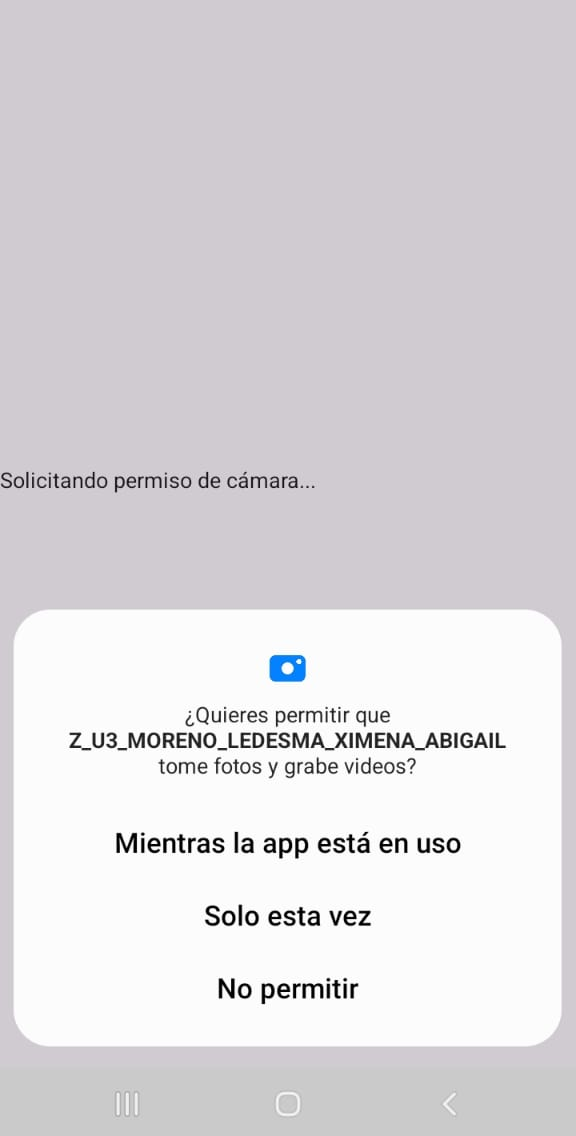
\includegraphics[width=160pt, height=260pt]{1.png}
\caption{Solicitud de permisos para el uso de cámara y galería.}
\label{fig:s1}
\end{figure}


Una vez concedidos los permisos, la aplicación presenta la opción de personalizar el entorno visual mediante un botón para seleccionar un fondo \textcolor{red}{\autoref{fig:s2}}. Al activarlo, se despliega la galería del dispositivo, donde la persona puede elegir entre diferentes imágenes disponibles \textcolor{red}{\autoref{fig:s3}}.
\begin{figure}[htbp]
\centering
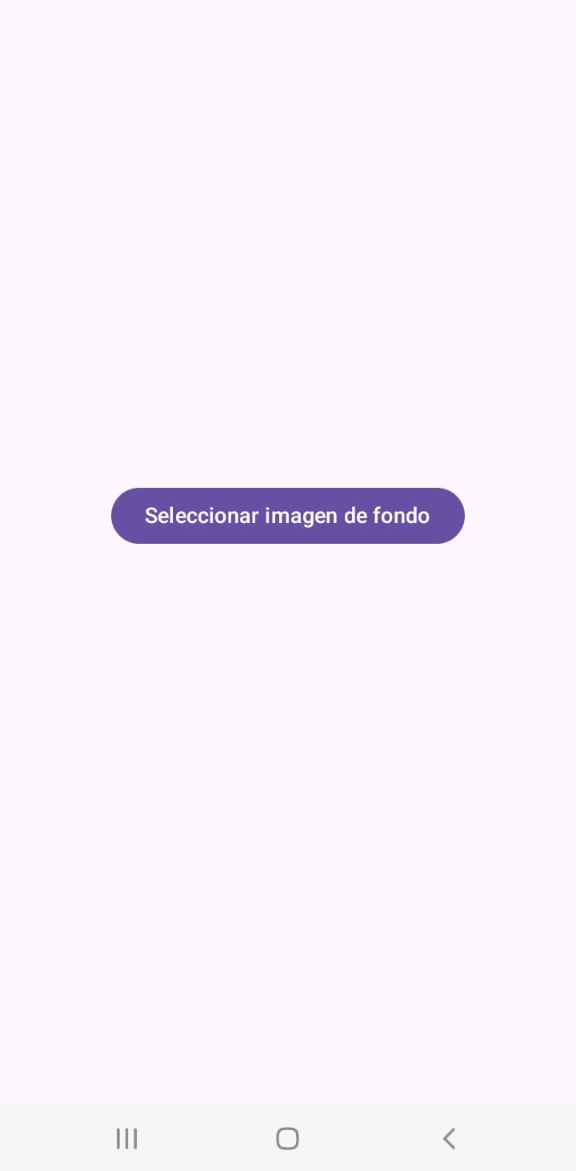
\includegraphics[width=160pt, height=260pt]{2.png}
\caption{Botón para seleccionar imagen de fondo.}
\label{fig:s2}
\end{figure}

\begin{figure}[htbp]
\centering
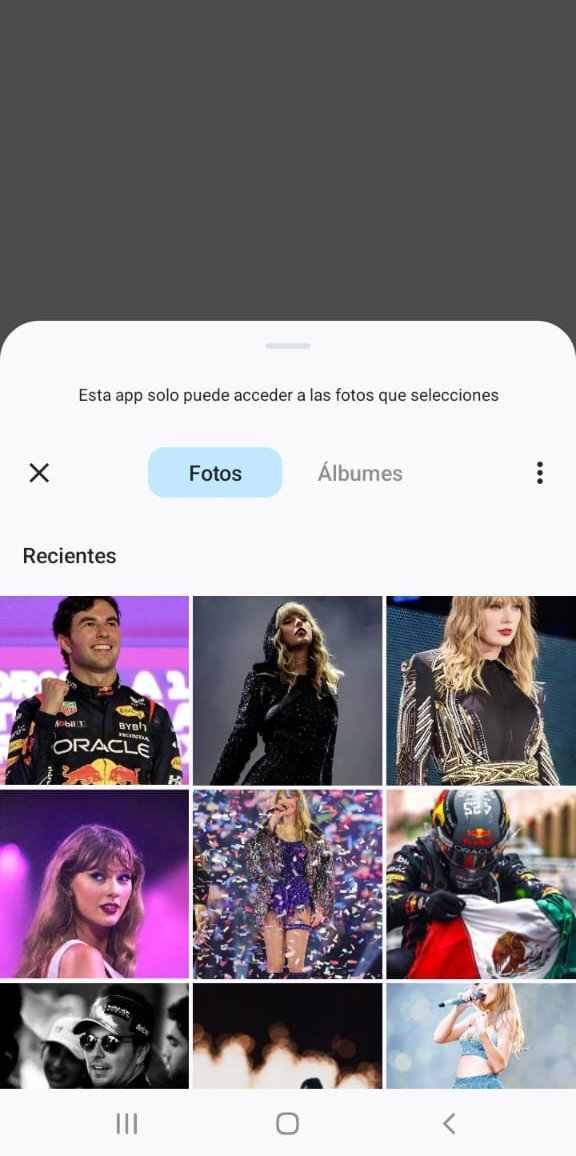
\includegraphics[width=160pt, height=250pt]{3.png}
\caption{Vista de la galería de imágenes para elegir fondo.}
\label{fig:s3}
\end{figure}

\newpage
Posteriormente, el sistema procesa la fotografía capturada, aplicando segmentación para aislar a la persona del fondo original. En la \textcolor{red}{\autoref{fig:s4}} se muestra el resultado final, donde la persona permanece en primer plano mientras se sustituye el fondo por la imagen seleccionada de la galería. Este procesamiento se realiza en tiempo real, garantizando una experiencia fluida.

\begin{figure}[htbp]
\centering
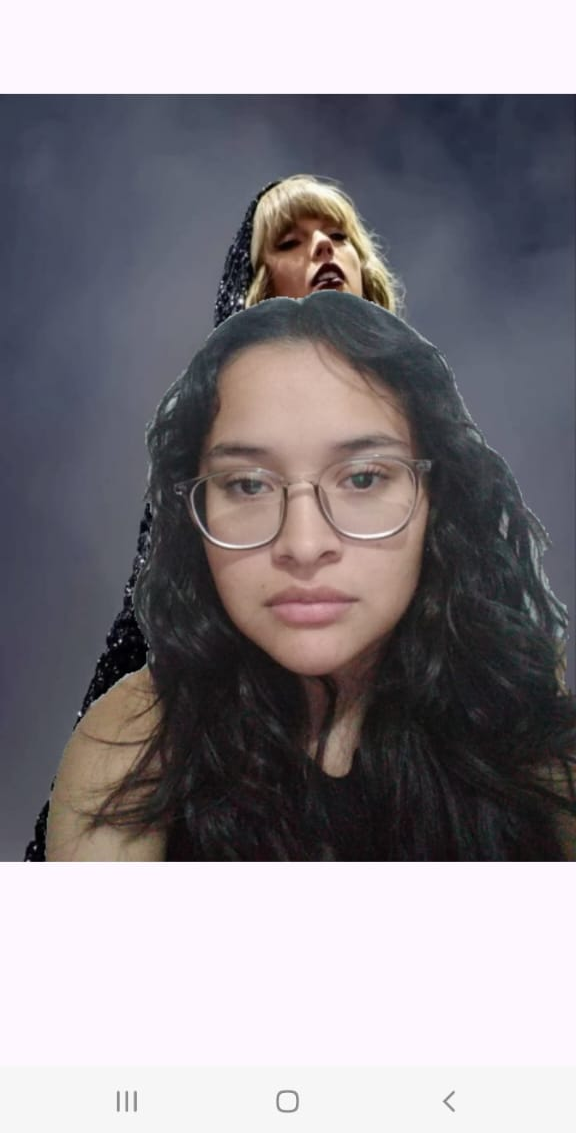
\includegraphics[width=160pt, height=250pt]{4.png}
\caption{Resultado de segmentación con la persona sobre el fondo seleccionado.}
\label{fig:s4}
\end{figure}


\newpage
\section{Conclusión}
En este trabajo se desarrolló una aplicación Android capaz de realizar segmentación de personas en tiempo real y reemplazo dinámico de fondo usando CameraX, ML Kit Selfie Segmentation y Jetpack Compose.En un inicio, se intentó usar el tutorial de Fritz AI, pero presentó dificultades por SDK desactualizado, dependencias incompatibles y falta de compatibilidad con interfaces modernas. Por ello, se tomó como referencia un video de Python sobre remoción de fondo con OpenCV, adaptando su lógica a Android y Compose.

La aplicación resultante permite seleccionar un fondo desde la galería y combinarlo en tiempo real con la persona capturada por la cámara. Cada frame se convierte de YUV a Bitmap RGB, se segmenta la persona y se renderiza sobre el fondo elegido.Haber trabajado con Jetpack Compose facilitó la creación de la interfaz, reduciendo código repetitivo, mejorando la modularidad y reutilización de componentes.

Las pruebas confirmaron que la segmentación y el reemplazo de fondo funcionan correctamente, mostrando el potencial de esta solución para efectos visuales, videollamadas y aplicaciones de realidad aumentada.

\printbibliography



\end{document}
